\documentclass[11pt]{article}

\usepackage[top=1.25in, bottom=1in, left=.8in, right=.8in]{geometry}

\usepackage{amsmath,amssymb,amsthm}
\usepackage{graphicx}
\usepackage{mwe}



%%%%%%%%%%%%%%%%%%%%%%%%%%%%%%%%%%%%%%%%%%%%%%
\begin{document}

\begin{flushright}
2018 SCHINDLER UCSC PHYS 133\\
\end{flushright}

\begin{center}
\noindent  \textbf{ \LARGE AC Circuits and Impedance}
\end{center}

\noindent In basic DC circuits, along with Kirchoff's laws, the fundamental equation is \textit{DC Ohm's Law},  
$ V = IR,$ 
relating the voltage and current across a resistor. 

In AC circuits, this gets generalized to \textit{AC Ohm's Law},
$ V = Iz$. 
It looks like the DC version, and plays a similar role, but actually more is going on here. In this context $V,I,z$ are all complex numbers.

You'll see why below.

\section*{Resistors, Capacitors, Inductors}
The three basic (passive, linear) ideal electronic components are the resistor, capacitor, and inductor. At any given time, each can have an instantaneous voltage $V(t)$, and an instantaneous current $I(t)$, across it. The relation between the instantaneous voltages and currents are determined by the electromagnetic physics of the components:

{
\begin{center}
\begin{tabular}{cc}
\raisebox{-.4\height}{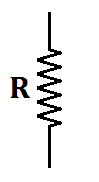
\includegraphics[scale=.3]{images/R.png} }
&
$V(t) = I(t) \, R$
\\
\raisebox{-.4\height}{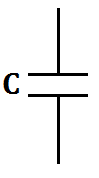
\includegraphics[scale=.3]{images/C.png} }
&
$C \, \dfrac{d V\!(t)}{dt} = I(t) $
\\
\raisebox{-.4\height}{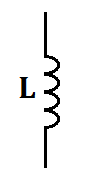
\includegraphics[scale=.3]{images/L.png} }
&
$V(t) = L \, \dfrac{d I(t)}{dt}$
\end{tabular}
\end{center}
}

\noindent For AC circuits, we will assume all voltages are oscillating sinusoidally, and these will turn into equations for the impedance.


\section*{Complex Exponentials and Oscillation}
\paragraph*{Oscillations.}
An oscillating signal is any signal of the form
$$ y(t)= A \, \cos(\omega t + \delta),$$
which is an arbitrary sinusoidal function. $A$ is called the \textit{amplitude}, and $\delta$ is called the \textit{phase shift}.

Due to Euler's identity $e^{i\theta} = \cos\theta + i\sin\theta$, this signal can also be written as
\begin{align*}
y(t) = \text{Re} \left( \, A e^{i\delta} \, e^{i\omega t}  \, \right)
   = \text{Re} \left( \, Y e^{i\omega t}  \, \right)
\end{align*}
where we have defined the complex number $Y = A e^{i\delta}$. $Y$ is called the \textit{complex amplitude} of the oscillation $y(t)$, and encodes both the amplitude and the phase by using a single complex number to represent two real numbers. Indeed, $|Y| = A$ and $\phi_Y = \delta$.

To simplify circuit analysis, we can treat all oscillations as complex, taking the real part only at the end. (This is possible when solving any system of linear differential equations with real coefficients.) This lets us forget about the instantaneous quantities $y(t)$, and work with the complex amplitudes $Y$.


\paragraph*{Complex numbers.} Recall that any complex number has the forms
\begin{align*}
 z &= \text{Re}(z) + i \, \text{Im}(z) \\
    & = |z| \, e^{i\phi_z}
\end{align*}
where
\begin{align*}
|z|^2 &= \text{Re}(z)^2 +  \text{Im}(z)^2
&
\phi_z &= \tan^{-1} \left( \tfrac{\text{Im}(z)}{ \text{Re}(z)} \right).
\end{align*}
You can think of $z$ as a vector in a plane, where the x-axis is the real part and the y-axis is the imaginary part. The \textit{magnitude} $|z|$ is the length of the vector, and the \textit{phase} $\phi_z$ (also called the \textit{argument} $\text{Arg}(z)$) is the angle from the +x-axis.

The \textit{complex conjugate} of $z$ is defined by $z^* = \text{Re}(z) - i \, \text{Im}(z)$. It is useful to know that $z^* z = |z|^2$.



\section*{AC Circuits}
By an AC circuit, we mean a circuit where everything is oscillating at a fixed frequency $f$. This corresponds to an angular frequency $\omega = 2\pi f$. Therefore, we assume that all voltages and currents in the circuit have the form
\begin{align*}
V_k(t) &= V_k e^{i\omega t}  &  I_k(t) &= I_k e^{i\omega t}
\end{align*}
where $k$ is a label for the voltages and currents at different spots. The quantities $V_k$ and $I_k$ are complex amplitudes (NOTE: in this notation $V_k$ and $V_k(t)$ are two different things, and the same goes for $I$). Each voltage and current has a different complex amplitude, but all have the same frequency of oscillation. The complex amplitudes ultimately tell us the amplitude and phase shift of the real oscillation.

Plugging the assumed form for $V(t)$ and $I(t)$ into the above equations for R, L, and C, we can cancel out the exponential factors, which leaves an equation for the complex amplitudes:

{
\begin{center}
\begin{tabular}{cc}
\raisebox{-.4\height}{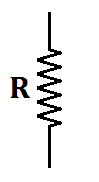
\includegraphics[scale=.3]{images/R.png} }
&
$ V = I \, R $
\\
\raisebox{-.4\height}{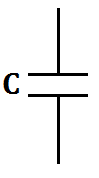
\includegraphics[scale=.3]{images/C.png} }
&
$ V = I \, (\frac{1}{i\omega C}) $
\\
\raisebox{-.4\height}{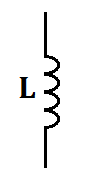
\includegraphics[scale=.3]{images/L.png} }
&
$ V = I \,(i \omega L) $
\end{tabular}
\end{center}
}

Each of these equations has the form
$$ V = I z ,$$
where all three quantities are complex numbers (and not functions of time). We call this equation \mbox{\textit{AC Ohm's Law}}. It states that, in AC circuits, the complex amplitudes of voltage and current oscillation across a (passive, linear) component are proportional.  The constant of proportionality $z$ is called the \textit{impedance} (also sometimes called the \textit{complex impedance} for emphasis). Notice that in general, the impedance of a component depends on frequency.



\section*{Impedance}
We have just deduced the complex impedances for an ideal resistor, capacitor, and inductor: 

{
\begin{center}
\begin{tabular}{clccc}
\raisebox{-.4\height}{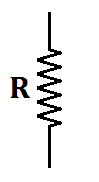
\includegraphics[scale=.3]{images/R.png} }
&
$z_R = R $
&
\raisebox{-.45\height}{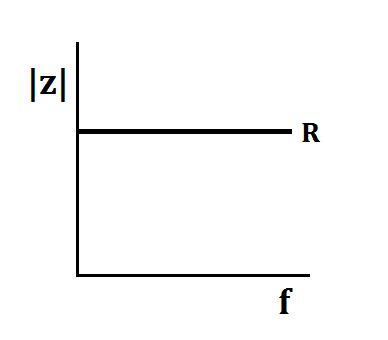
\includegraphics[scale=.3]{images/Rg.png} }
&
\raisebox{-.45\height}{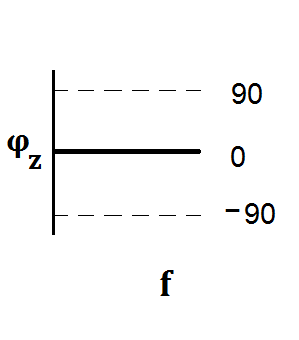
\includegraphics[scale=.3]{images/Rg2.png} }
&
freq independent
\\
\raisebox{-.4\height}{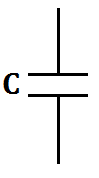
\includegraphics[scale=.3]{images/C.png} }
&
$z_C = \dfrac{1}{i\omega C} $
&
\raisebox{-.45\height}{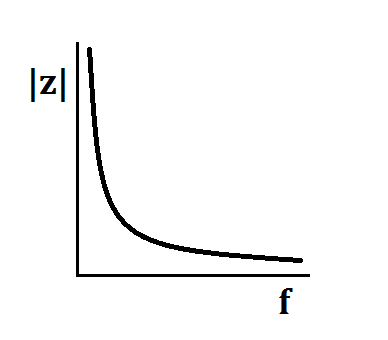
\includegraphics[scale=.3]{images/Cg.png} }
&
\raisebox{-.45\height}{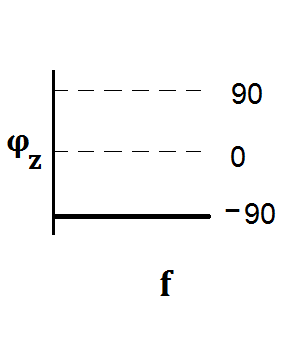
\includegraphics[scale=.3]{images/Cg2.png} }
&
blocks lo f ... passes hi f
\\
\raisebox{-.4\height}{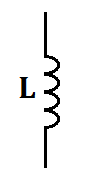
\includegraphics[scale=.3]{images/L.png} }
&
$z_L = i\omega L $
&
\raisebox{-.45\height}{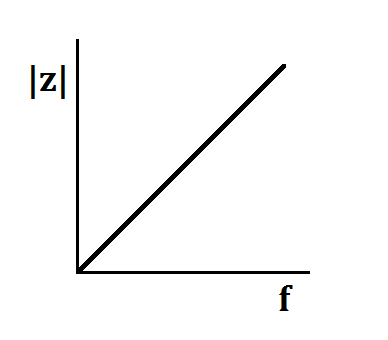
\includegraphics[scale=.3]{images/Lg.png} }
&
\raisebox{-.45\height}{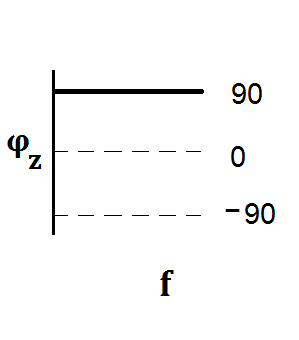
\includegraphics[scale=.3]{images/Lg2.png} }
&
passes lo f ... blocks hi f
\end{tabular}
\end{center}
}


It is not hard to show (from Kirchoff's laws) that impedances combine just like DC resistances. In particular:

\begin{center}
\begin{tabular}{ccc}
series  & $\;\;\;\;\;\;$ & parallel  \\
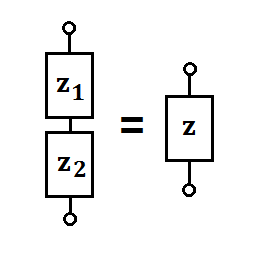
\includegraphics[scale=.3]{images/series.png} &   &
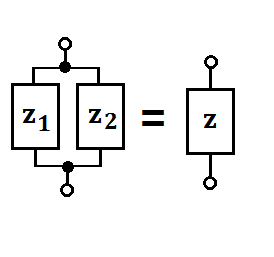
\includegraphics[scale=.3]{images/parallel.png} \\
$z = z_1 + z_2$    &   & $\frac{1}{z} = \frac{1}{z_1} + \frac{1}{z_2}$ 
\end{tabular}
\end{center}
In this way, more complicated functions $z(f)$ can be built up from the basic impedances.

In general, every passive circuit element will have some impedance $z(f)$, which will vary as a function of frequency. For circuit elements containing a combination of resistance, capacitance, and inductance, $z(f)$ may be a complicated function. This impedance can be measured by measuring the complex amplitudes $V$ and $I$ across a circuit element, since $z = V/I$.

\paragraph*{Example.} A resistor in series with an inductor has an impedance $z = R + i\omega L$. It follows that the magnitude is $|z| = \sqrt{R^2 + \omega^2 L^2}$ and that the phase is $\phi_z = \tan^{-1} (\frac{\omega L}{R})$. All three quantities are functions of frequency $f$, where $\omega = 2\pi f$.


\clearpage
\section*{Phys 133 Experiment}
\begin{center}
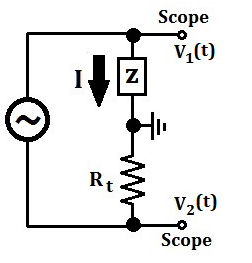
\includegraphics[scale=.5]{images/testcircuit.png}
\end{center}

The circuit depicted above can be used to measure the impedance of the circuit element \mbox{labelled $z$}. \mbox{$R_t$ is} a known resistance ($t$ stands for ``test"), and for simplicity let's denote $R_t=R$ for now.

In its default mode, the oscilloscope screen will display graphs of $V_1(t)$ and $V_2(t)$. For this experiment, change the scope setting to \texttt{CH2 INVERT ON}; now the scope will display $V_1(t)$ and $-V_2(t)$ (note the negative sign, meaning that the graph is flipped upside down). This is not necessary, but it is convenient.

$V_1(t)$ is the voltage across the unknown box, and since $-V_2(t)=I(t)\, R$, the function $-V_2(t)$ is just a vertically stretched version of the current. Therefore you can visualize the scope's yellow curve as the voltage across the box, and the blue curve as the current through the box.

From the functions $V(t)$ displayed, we want to extract the complex amplitudes of oscillation. Using the scope's \texttt{MEASURE} menu, we have the ability to measure the real amplitude of each oscillation, and the relative phase difference between the two oscillations. This is enough to extract the impedance.

Denote the complex amplitudes by $V_1$, $V_2$, and $I$. \mbox{By definition}, $z= V_1/I$. But $I=(-V_2)/R$. Therefore
\begin{align*}
z = \frac{V_1 R}{(-V_2)} = \frac{|V_1| R}{|-V_2|} \, e^{i (\phi_{(V_1)} - \phi_{(-V_2)})} = \frac{|V_1| R}{|-V_2|} \, e^{i \delta } 
\end{align*}
where $\delta$ is defined as the relative phase difference between $V_1(t)$ and $-V_2(t)$. 

We can directly measure $|V_1|$, $|-V_2|$, and $\delta$ using the scope, and directly measure $R$ using an ohmmeter, so the formula 
\begin{align*}
z = \frac{|V_1| R}{|-V_2|} \, e^{i \delta } 
\end{align*}
experimentally defines the complex impedance. In particular
\begin{align*}
|z| &= \frac{|V_1| R}{|-V_2|}  &
\phi_z  &=  \delta
\end{align*}

The preceding method determines $z$ at a fixed frequency. By sweeping through a range of frequencies, one can map out the function $z(f)$.






\end{document}
